\documentclass[a4paper]{scrartcl}
\usepackage{titling}

% LANGUAGE and LOCALE
\usepackage[USenglish,ngerman]{babel} % Deutsches Wörterbuch usw.
\newcommand{\en}[1]{\selectlanguage{USenglish}#1\selectlanguage{ngerman}}

% FONT
\usepackage[T1]{fontenc}
\usepackage[utf8]{inputenc}
\usepackage[babel=true]{microtype} % after babel
\usepackage{lmodern}
%\usepackage{times}
\makeatletter
\g@addto@macro\@verbatim{\microtypesetup{activate=false}}
\makeatother

% ENUMERATE and ITEMIZE
\usepackage{enumerate}
\usepackage{paralist}

% SCIENCE and MATH
\usepackage{amsmath}
\usepackage{amssymb}
\usepackage{icomma}
%\usepackage{units}
\usepackage{xfrac} % Brüche im Stil von ½ (\sfrac)

% PROGRAMMING
\usepackage{algorithm}
\usepackage[noend]{algpseudocode}

% TABLES
%\usepackage{array}
%\usepackage{multicol}	
%\usepackage{dcolumn}
%\usepackage{slashbox} % diagonale Linie in Tabellenzelle
%\usepackage{tabularx}

% LINKS and REFS
\usepackage[obeyspaces]{url}
\usepackage{hyperref}
\usepackage{todonotes} % todos..

% BIBLIOGRAPHY
\usepackage[style=german,german=quotes]{csquotes}
\usepackage[style=alphabetic,backend=biber,babel=hyphen,maxbibnames=10]{biblatex}
%\usepackage[authordate,backend=biber,babel=hyphen]{biblatex-chicago} 
\bibliography{hgraph.bib}

% FORMATING
\usepackage{enumitem} % nicer itemize
\usepackage{listings}
\usepackage{color}
\definecolor{mygreen}{rgb}{0,0.6,0}
\definecolor{mygray}{rgb}{0.5,0.5,0.5}
\definecolor{mymauve}{rgb}{0.58,0,0.82}
\lstset{ %
  backgroundcolor=\color{white},   % choose the background color; you must add \usepackage{color} or \usepackage{xcolor}
  basicstyle=\scriptsize,        % the size of the fonts that are used for the code
  breakatwhitespace=false,         % sets if automatic breaks should only happen at whitespace
  breaklines=true,                 % sets automatic line breaking
  captionpos=b,                    % sets the caption-position to bottom
  commentstyle=\color{mygreen},    % comment style
  deletekeywords={...},            % if you want to delete keywords from the given language
  escapeinside={\%*}{*)},          % if you want to add LaTeX within your code
  extendedchars=true,              % lets you use non-ASCII characters; for 8-bits encodings only, does not work with UTF-8
  frame=single,                    % adds a frame around the code
  keepspaces=true,                 % keeps spaces in text, useful for keeping indentation of code (possibly needs columns=flexible)
  keywordstyle=\color{blue},       % keyword style
  language=Haskell,                % the language of the code
  morekeywords={*,Graph,Adj,Attr,Density,MaxDivergence,L,expand,filterLayer,...},            % if you want to add more keywords to the set
  numbers=left,                    % where to put the line-numbers; possible values are (none, left, right)
  numbersep=5pt,                   % how far the line-numbers are from the code
  numberstyle=\tiny\color{mygray}, % the style that is used for the line-numbers
  rulecolor=\color{black},         % if not set, the frame-color may be changed on line-breaks within not-black text (e.g. comments (green here))
  showspaces=false,                % show spaces everywhere adding particular underscores; it overrides 'showstringspaces'
  showstringspaces=false,          % underline spaces within strings only
  showtabs=false,                  % show tabs within strings adding particular underscores
  stepnumber=1,                    % the step between two line-numbers. If it's 1, each line will be numbered
  stringstyle=\color{mymauve},     % string literal style
  tabsize=2,                       % sets default tabsize to 2 spaces
  title=\lstname                   % show the filename of files included with \lstinputlisting; also try caption instead of title
}
\usepackage{anysize} % Makros zum Einstellen der Seitenränder
\parindent0em % Keine amerikanische Einrückung am Anfang von Paragraphen
\clubpenalty = 10000  % Schusterungen bestrafen
\widowpenalty = 10000 % Hurenkinder bestrafen
\displaywidowpenalty = 10000

% math commands
\newcommand{\trans}[1]{{#1}^\intercal}
\newcommand{\abs}[1]{\left\vert #1 \right\vert}
\newcommand{\card}[1]{\left\vert #1 \right\vert} % cardinality
\newcommand{\norm}[1]{\left\Vert #1 \right\Vert}

\newcommand{\condset}[2]{\ensuremath{\left\lbrace #1\vphantom{#2}\right.\left\vert\; #2 \vphantom{#1}\right\rbrace}}

\newcommand{\setR}{\mathbb{R}}
\newcommand{\setN}{\mathbb{N}}

\DeclareMathOperator*{\argmin}{\arg\min}
\DeclareMathOperator*{\argmax}{\arg\max}

\hyphenation{IEEE} % hyphenation of default language
\begin{hyphenrules}{USenglish} % hyphenation of secondary language
  \hyphenation{IEEE}
\end{hyphenrules}

\begin{document}

\title{\en{Densely Connected Biclusters}}
\author{Stefan Dresselhaus \and Thomas Pajenkamp}
\date{\today} % TODO: Abgabedatum
\newcommand{\thesemester}{Wintersemester 2013/14}
\newcommand{\thecategory}{Programmierprojekt}
\newcommand{\thecourse}{Parallele Algorithmen und Datenverarbeitung}


%
% Deckblatt
%
\begin{titlepage}
  \begin{center} 
    \mbox{}
     \vspace{1cm}\\
     {\Huge \textbf{\thetitle}} \\[3em]
     {\huge \theauthor} \\[4em]
     {\Large \thecourse}\\[1em]
     {\Large \thecategory{} im \thesemester}\\[1em]
     
     \vspace{3cm}
     
     {\LARGE Universität Bielefeld -- Technische Fakultät}\\[2em]
     {\large \thedate}
  \end{center}
\end{titlepage}
%
% Inhaltsverzeichnis
%
%\setcounter{page}{1}
\microtypesetup{protrusion=false}
\tableofcontents
\microtypesetup{protrusion=true}

\listoftodos
\newpage

\section{Zielsetzung des Projekts}

Im Rahmen dieses Programmierprojekts wurde ein Programm entworfen und entwickelt, um \en{Densely Connected Biclusters}, im weiteren DCB, in einem biologischen Netzwerk zu ermitteln. Bei DCB handelt es sich um Teilgraphen eines Netzwerks, dessen Knoten untereinander hoch vernetzt sind und Objekte mit ähnlichen Eigenschaften repräsentieren. \par
Die Suche nach DCB ist ein NP-schweres Problem. Da mit einem geeigneten Algorithmus jedoch voneinander unabhängige Lösungspfade einzeln verfolgt werden können, ist das Problem gut für eine parallele Berechnung geeignet, wodurch die Gesamtlaufzeit stark reduziert werden kann. Zudem sind  real verwendete biologische Netze üblicherweise nur schwach vernetzt. Daher können durch die Forderung nach einer hohen Konnektivität der DCB viele Lösungskandidaten schnell ausgeschlossen werden und die schlimmstenfalls nichtdeterministisch polynomielle Laufzeit findet kaum Anwendung. \par

%TODO ein bisschen biologische Motivation?
% ... Sind wir Biologen? :p

\en{
\subsection{Densely Connected Biclusters}
\label{dcb}
}

Ausgangsbasis ist ein ungerichteter ungewichteter Graph $G = (V, E)$, dessen Knoten $n \in V$ mit jeweils $p$ Attributen versehen sind. Jedem Knoten $n$ ist zu jedem Attribut $i$ ein numerischer Wert $a_{ni}$ zugewiesen. \par
Ein DCB $D_k = (V_k, E_k)$ ist ein Teilgraph von $G$, der durch die Parameter $\alpha \in [0, 1]$, $\delta \in \setN$ und $\omega \in \setR^p$ beschränkt wird und die folgende drei Eigenschaften erfüllt.
\begin{itemize}
\item Der Teilgraph ist zusammenhängend.
\item Die Dichte des Teilgraphen unterschreitet einen Schwellenwert $\alpha$ nicht, also $\frac{2 \cdot \card{E_k}}{\card{V_k}(\card{V_k}-1)} \geq \alpha$.
\item Für mindestens $\delta$ Attribute liegen die Werte aller Knoten des Teilgraphen höchstens $\omega_i$ auseinander. Anders ausgedrückt
\begin{equation*}
\delta \leq \card{\condset{1\leq i \leq p}{\omega_k \geq \left(\max_{n\in V_k} a_{ni} - \min_{n\in V_k} a_{ni}\right)}} \text{\@.}
\end{equation*}
\end{itemize}


\section{Wahl der Programmiersprache und Konzept der Parallelisierung}

Die Wahl der Programmiersprache zur Verwirklichung des Projekts beeinflusst stark die Methoden der Programmierung und die Art der Parallelisierung. Klassischerweise werden für sequentielle und parallele Programme gleichermaßen imperative Sprachen wie C(++), Fortran oder auch Java verwendet, wofür Erweiterungen zur parallelen Programmierung existieren oder einige Werkzeuge direkt in die Sprache eingebaut sind. Bekannte Ansätze hierfür sind MPI und openMP. \par
Unser Projekt geht in eine etwas andere Richtung. Bei imperativer Programmierung muss ein großes Augenmerk auf die Vermeidung unerwünschter wechselseitiger Beeinflussungen verschiedener Threads und Prozesse gelegt werden, die fehlerhafte Rechenergebnisse zur Folge haben. Außerdem muss bei der Thread-/Prozesskommunikation immer die Gefahr von Verklemmungen beachtet werden, die schlimmstenfalls zu einem kompletten Stillstand der Programmausführung führen. Beide Probleme sind schwierig zu detektieren und zu lokalisieren.\par
Die genannten klassischen Probleme des Parallelrechnens können mit pur funktionaler Programmierung gut vermieden werden. Nebenbedingungen treten in pur funktionalem Programmcode (einen korrekten Compiler/Interpreter vorausgesetzt) garantiert nicht auf. Da das DCB-Problem bis auf das Einlesen der Eingabedaten und die Ausgabe pur funktional realisierbar ist, ist es optimal für eine derartige Implementierung geeignet Die konkrete Wahl der funktionalen Programmiersprache fiel auf \emph{Haskell}. \par
\medskip
Für Haskell wurden Bibliotheken entwickelt, die eine einfache und effiziente Programmierung paralleler Programme erlauben. Wir verwenden das Paket \emph{parallel} in Verbindung mit \emph{repa}-Arrays. Durch \emph{parallel} können geeignete Algorithmen mit wenig Aufwand, aufgeteilt werden. Dabei werden Funktionsaufrufe unevaluiert in einem Array gespeichert und dort von freien Threads abgearbeitet. Diese Technik nennt man Work-Stealing und die noch nicht ausgewerteten Funktionen werden in Haskell \emph{Sparks} genannt. Man kann sich dies als einen auf den Funktionsaufruf beschränkten light-weight Thread vorstellen -- mit weniger Overhead. Die \emph{repa}-Arrays bieten Funktionen, um die einzelnen Elemente eines Arrays parallel zu berechnen. Mit diesen Techniken lässt sich sequentieller Programmcode einfach parallelisieren, da hierfür nur wenige Änderungen im Programmcode erforderlich sind. Es müssen lediglich die Berechnungsfunktionen an die parallelisierende Funktion übergeben und die Funktion zur Auswertung der Arrayelemente ausgetauscht werden. \par
\medskip
Zwei wichtige Punkte müssen dennoch beachtet werden. Zum einen verwendet Haskell das Konzept \emph{\en{Lazy Evaluation}}. Befehle werden immer nur soweit berechnet, wie sie an anderer Stelle benötigt werden. Dadurch entstehen manchmal zur Laufzeit große Bäume nur teilweise ausgewerteter Befehle, welche die Ausführungszeit durch eine hohe Garbage-Collector-Auslastung stark negativ beeinflussen. Es muss demnach darauf geachtet werden, die Berechnung später ohnehin erforderlicher Funktionen frühzeitig zu erzwingen. Zum anderen ist die Anzahl der Sparks standardmäßig nicht begrenzt, sodass auch hier zu große Arrays entstehen können, deren Abarbeitung allerdings im Verlaufe des Programms durch o.\,g. Lazy Evaluation evtl.\ gar nicht erforderlich ist. Daher beschränken wir die Anzahl der möglichen Sparks (und somit der maximal möglichen Worker-Threads) auf 1000. Erwähnenswert ist noch, dass diese Technik \emph{nicht} von Hyper-Threading profitiert,da kein Kontextwechsel der Threads nötig ist, und wir somit 1000 \glqq echte\grqq \ Kerne für eine maximale Auslastung benötigen. Die obere Grenze wird eher durch Amdahls Gesetz, denn durch die verfügbaren Kerne beschränkt.\par


\section{Der Algorithmus}

Für die Darstellung des Eingabegraphen, in dem die DCB gesucht werden, verwenden wir eine Adjazenzmatrix. Die anschließende Laufzeitbetrachtung bezieht sich auf diese Datenstruktur. \par
Der DCB-Algorithmus besteht aus einer Vorverarbeitungsphase, in der Cluster-Seeds aus 2 jeweils verbundenen Knoten generiert werden, und einer anschließenden Expansion dieser Seeds unter Berücksichtigung der in Abschnitt~\ref{dcb} vorgestellten Nebenbedingungen (Constraints). Diese Cluster (im Folgenden Graphen genannt) bestehen zu Anfang aus genau 2 Knoten, die sämtliche Bedingungen erfüllen. Eine erste Optimierung findet nun statt, da es nach diesem Schritt auch verbundene Knoten geben kann, die nicht zur initialen Bildung der Graphen beigetragen haben. Diese Paare können im Folgenden komplett ausgeschlossen werden, da sie die Attributsbedingung nicht erfüllen können\footnote{Ein Graph aus 2 verbundenen Knoten ist immer maximal dicht und zusammenhängend.}. Folglich würde jeder Graph mit diesem Knotenpaar insgesamt auch gegen selbige Attributsbedingung verstoßen. Alle hiervon betroffenen Kanten können somit aus der Adjazenzmatrix gelöscht werden.\par

\begin{figure}[h!]
 \centering
 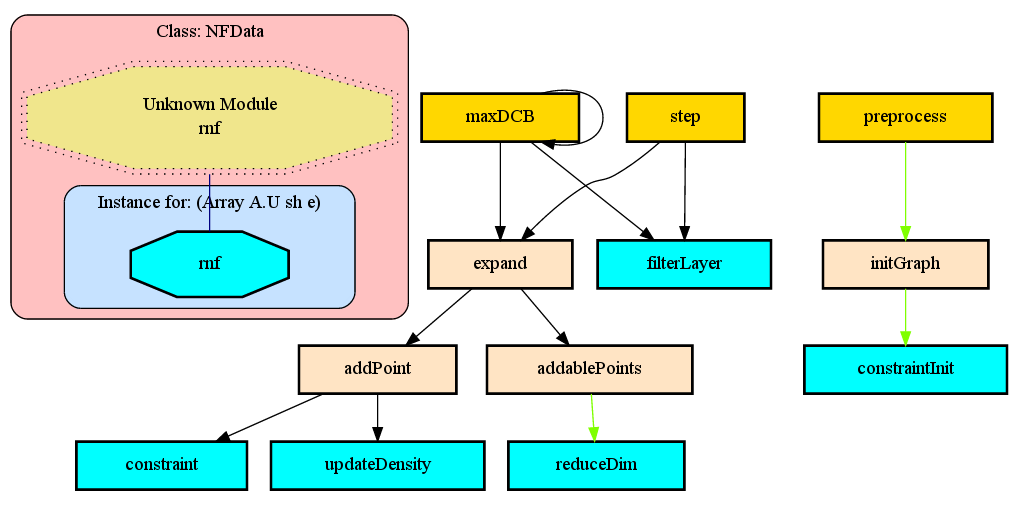
\includegraphics[scale=0.5,keepaspectratio=true]{./img/DCB-Module.png}
 % DCB-Module.png: 1024x512 pixel, 96dpi, 27.09x13.54 cm, bb=0 0 768 384
 \caption{Übersicht über die Hierarchie des DCB-Moduls. Gelb hinterlegte Funktionen sind nach außen hin sichtbar.}
 \label{fig:DCB-Overview}
\end{figure}

Wir exportieren 2 Funktionen nach außen, die in der Lage sind, den Graphen zu expandieren: \texttt{step} und \texttt{maxDCB}. \texttt{step} liefert alle möglichen expandierten Graphen aus einer Liste von bestehenden DCB -- allerdings verliert man somit alle Graphen, die nicht expandiert werden konnten. Als Ergebnis hat man eine gewisse Mindestzahl an Knoten im Graphen. Da die Seeds mit 2 Knoten beginnen, man aber z.\,B. alle DCB mit 4 Knoten oder mehr haben möchte, kann man \texttt{step} so häufig aufrufen, dass alle Graphen mit weniger Knoten gar nicht zurückgegeben werden. Wir verwenden dies in unserem Algorithmus einmalig, da wir nur Cluster mit 3 oder mehr Knoten zurückliefern.\par
\medskip
Die Funktion \texttt{maxDCB} übernimmt die eigentliche Berechnung, sodass wir diese im Detail besprechen. Zunächst jedoch geben wir einen kleinen Überblick über die Hilfsfunktionen im Hintergrund:
\begin{description}[style=multiline,leftmargin=2.75cm,font=\bfseries]
 \item[filterLayer] filtert eine Menge von $s$ Graphen der Größe $m$, indem es Duplikate herausfiltert. \\ Laufzeit: $\mathcal{O}(m \cdot s \log s)$.
 \item[constraint] überprüft, ob der Graph noch die Constraints erfüllt und wenn ja, wie diese aussehen. \\ Laufzeit: $\mathcal{O}(k)$ bei $k$ Attributen, da die Maximal- und Minimalwerte des Graphen tabelliert werden.
 \item[updateDensity] errechnet die Änderung der Dichte des Graphen anhand des hinzuzufügenden Punktes. \\ Laufzeit: $\mathcal{O}(m)$ bei $m$ Knoten im Ursprungsgraph, da die Graphendichten gespeichert werden.
 \item[reduceDim] ist eine interne Hilfsfunktion, die eine Dimension einer Array-Shape verwirft. \\ Laufzeit: $\mathcal{O}(1)$.
 \item[addablePoints] traversiert die Adjazenzmatrix und liefert alle mit einem Graphen verbundenen Knoten, die nicht selbst im Graphen enthalten sind. \\ Laufzeit: $\mathcal{O}(n \cdot m)$ bei $m$ Knoten im Ursprungsgraphen und einer Adjazenzmatrix $n\times n$.
 \item[addPoint] erweitert wenn möglich einen bestehenden Graphen um einen Knoten, indem es zunächst ein \texttt{updateDensity} durchführt und anschließend mittels \texttt{constraint} alle Nebenbedingungen überprüft. \\ Laufzeit: $\mathcal{O}(k + m)$, falls die Density-Constraint erfüllt bleibt, sonst $\mathcal{O}(k)$.
 \item[expand] wendet \texttt{addPoint} auf alle Ergebnisse von \texttt{addablePoints} an.\\
 Laufzeit: $\mathcal{O}(n \cdot m \cdot (k + m))$ im worst-case einer voll besetzten Adjazenzmatrix. In der Praxis sind die Eingabegraphen kaum vernetzt und die Attributzahl $k$ ist klein, sodass sich die average-case-Laufzeit unter Berücksichtigung der alternativen Laufzeit von \texttt{addPoint} an $\mathcal{O}(n \cdot m \cdot k) \approx \mathcal{O}(n \cdot m)$ annähert.
 
\end{description}

\begin{lstlisting}[caption={Die maxDCB-Funktion},label=lst:maxDCB]
-- | Calculates all maximum DCB. A maximum DCB is a densely connected bicluster that
--   cannot be expanded by any additional node without breaking the constraints.
--   
--   This function does return the seed graphs themselves if they cannot be expanded.
maxDCB :: [Graph] -> Adj -> Attr -> Density -> MaxDivergence -> Int -> [Graph]
maxDCB [] _ _ _ _ _ = []
maxDCB gs adj attr dens maxDiv minHit =
    let next = L.map (expand adj attr dens maxDiv minHit) gs
                     +|| (parBuffer 1000 rdeepseq)
        (maximal, expandable) = part (\_ rm -> rm == []) (zip gs next)
        expandable' = filterLayer $ concat expandable
        -- Divide solutions into expandable solutions and maximum solutions.
        -- Expandable solutions yield a result via the 'expand' function.
    in maxDCB expandable' adj attr dens maxDiv minHit L.++ maximal
    -- append maximum solutions of prospective function calls and maximum solutions
    -- of this iteration
\end{lstlisting}

Der rekursive Funktionsaufruf findet in Zeile~14 statt. Hier werden iterativ alle expandierbaren Möglichkeiten evaluiert bis sie maximal erweitert sind und an die nicht erweiterbaren Graphen angehängt. In den Zeilen~8/9 wird die Expansion auf den Eingabegraphen \texttt{gs} parallel in einem Puffer von höchstens 1000 parallelen Anweisungen ausgeführt. Die Strategie, welche wir für die parallele Evaluation verwenden, lautet \texttt{rdeepseq}. Dadurch werden diese Graphen direkt vollständig ausgewertet und müssen nicht (z.\,B. durch Lazy Evaluation) nachberechnet werden.\par
\medskip
Anschließend partitionieren wir die expandierten Graphen in maximal erweiterte und in weiter expandierbare (Z.~10). Letztere filtern wir noch (Z.~11) nach Duplikaten, um redundante Weiterberechnung (und damit einen erhöhten Rechenaufwand) zu vermeiden. Zurückgeliefert werden somit alle Graphen, die maximal expandiert sind. \par
\medskip
Die Funktion \texttt{expand} wird letztendlich für jeden Graphen genau einmal aufgerufen. Der Rechenaufwand der $m$-ten Expansionsstufe mit $s$ Graphen ist zusammen mit der Filterung doppelter Graphen $\mathcal{O}(s m \cdot (n (k+m)+ \log s))$, für schwach vernetzte Eingabegraphen eher $\mathcal{O}(s m \cdot (n k + \log s))$. $k$ ist die Anzahl an Attributen und $n$ die Größe der Adjazenzmatrix. Allerdings wächst die Anzahl der Graphen pro Iteration im ungünstigsten Fall exponentiell an, woraus sich die Schwierigkeit des Problem als NP-schwer ergibt. In schwach vernetzten Eingabegraphen ist jedoch zu erwarten, dass die anfänglichen Seed-Graphen kaum erweitertbar sind, wodurch sich der gesamte Rechenaufwand stark reduziert. Dennoch besteht viel Potential zur Parallelisierung der Berechnung zur Verkürzung der Rechenzeit.

\section{Ausführung und Auswertung}
%TODO
Amdahls Gesetz, Minskys Vermutung\\
Nach jedem Erweiterungsschritt: Sammeln und Aufgaben neu verteilen $\rightarrow$ Kommunikation

\section{Fazit}
%TODO
Wir sind toll.

\newpage
\printbibliography[heading=bibintoc]

\end{document}